\documentclass[14pt]{beamer}
\usepackage[T2A]{fontenc}
\usepackage[utf8]{inputenc}
\usepackage[english,russian]{babel}
\usepackage{tikz}
\usepackage[european,cuteinductors,smartlabels]{circuitikz}

\usepackage{amssymb,amsfonts,amsmath,mathtext}
\usepackage{amssymb}
\usepackage{cite,enumerate,float,indentfirst}
\usepackage{cancel}
\usepackage{csquotes}
\newcommand{\quotes}[1]{``#1''}

%\usepackage{pgfplots}
%\usepackage[left=1cm,right=1cm, top=1cm,bottom=1cm,bindingoffset=0cm]{geometry}

% Beamer — верстаем презентации  https://habrahabr.ru/post/145523/ 
\graphicspath{{images/}}

\usetheme{Pittsburgh}
\usecolortheme{whale}

\setbeamercolor{footline}{fg=blue}
\setbeamertemplate{footline}{
\leavevmode%
\hbox{%
\begin{beamercolorbox}[wd=.333333\paperwidth,ht=2.25ex,dp=1ex,center]{}%
Прокшин А.Н. и др.
\end{beamercolorbox}%
\begin{beamercolorbox}[wd=.333333\paperwidth,ht=2.25ex,dp=1ex,center]{}%
Санкт-Петербург, 2019
\end{beamercolorbox}%
\begin{beamercolorbox}[wd=.333333\paperwidth,ht=2.25ex,dp=1ex,right]{}%
Стр. \insertframenumber{} из \inserttotalframenumber \hspace*{2ex}
\end{beamercolorbox}}%
\vskip0pt%
}

\newcommand{\itemi}{\item[\checkmark]}

	\usefonttheme[onlymath]{serif} % в формулах использовать текст с засечками
\begin{document}
\title{\small{Создание и апробирование лабораторной установки по учебному курсу Микроконтроллеры по теме \enquote{Генерация векторного ШИМ для управления трехфазным асинхронным двигателем}.}}
\author{\small{%
\emph{авторы:}~Василенко Виктор Андреевич\\%
\emph{}~Вербова Алина\\
\emph{}~Илюшин Антон Геннадьевич\\
\emph{}~Маслов Иван Андреевич\\
\emph{}~Прокшин Артем Николаевич\\% 
\emph{}~Халявин Дмитрий Игоревич}}



\institute{Санкт-Петербургский государственный электротехнический университет «ЛЭТИ» им. В.И. Ульянова (Ленина)}
\vspace{30pt}%
%Санкт-Петербургский государственный электротехнический университет\\
%«ЛЭТИ» им. В.И. Ульянова (Ленина)

\vspace{60pt}%

%\date{\small{Санкт-Петербург, 2019}}

\AtBeginSection{
	\begin{frame}
		\frametitle{Содержание}
		\tableofcontents[currentsection]
	\end{frame}
}

\begin{frame}
\titlepage	
\end{frame}

%\begin{frame}
%        \frametitle{Содержание}
%        \tableofcontents[currentsection] 
%\end{frame}
\begin{frame}
\frametitle{\small Цели, к которым стремились при реализации курса} 
\begin{itemize}
\item упрощение системы управления с использованием ковариантных и контравариантных координат;
\item использование дипломных проектов студентов предыдущих выпусков;
\item создание лабораторных стендов по тематике кафедры с перспективой на использование российских разработок;
\item использование свободного open-source программного обеспечения;
\item оформление УМКД;
\item ... будет сформулирована в результатах.
\end{itemize}
\end{frame}

\begin{frame}
\frametitle{\smallвнутренние ресурсы, на которые опирались}
\begin{itemize}
	\itemНа кафедре есть курсы по управлению приводом с помощью контроллеров ОМРОН; 
	\itemесть дешевые микроконтроллеры(SoC); увеличилась скорость, разрядность, есть функции управления эл.двигателями; 
	\itemпредыдущий курс \enquote{решение интерфейсных задач с помощью микроконтроллера at89} Кекконен А.В.,Тимофеев А.А.,который выполняется на asm,C в ``Keil''(8 установок); 
\itemобсуждалось (приводчикам нужны приводы) с Татаринцевым Н.И., Беловым М.П.;
\itemподелили:Татаринцев --двигатель постоянного тока, Прокшин -- асинхронный двигатель.  
\end{itemize}
\end{frame}


\begin{frame}
\frametitle{\smallпрограммы -- бесплатно}
\begin{itemize}
	\item в ОС Linux всё необходимое присутствует  ``из-коробки'':
		\begin{itemize}
		\item кросс-компилятор arm-none-eabi-gcc
		\item компилятор для ``родной'' системы gcc, g++
		\item  java-1.8.0-openjdk;
		\end{itemize}
	\item эти компиляторы возможно запускать в среде эмуляции Линукс(cygwin) в ОС Windows;
	\item STM выкупила  и сделала Atollic Studio бесплатным
		для своих микроконтроллеров. \href{atollic.com}{Atollic Studio} работает на всех ОС;
	\item www.ac6.fr выпускает бесплатный компилятор \href{www.openstm32.org}{System Workbench} 
на среде Eclipse и работает на всех операционных системах.
\end{itemize}
\end{frame}


\begin{frame}
\frametitle{\smallоборудование -- дешево} 
\begin{figure}
\begin{center}
\begin{minipage}[h]{0.5\linewidth}
\center{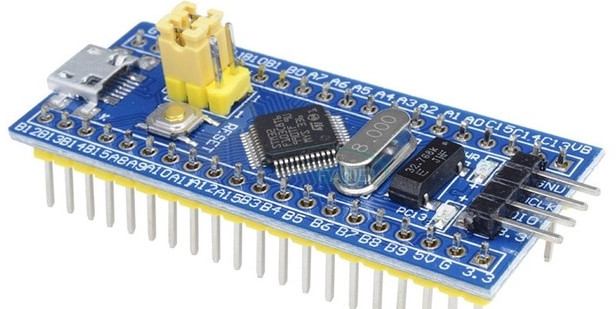
\includegraphics[width=1\linewidth]{stm32f103c8t6.jpg}}  \\
\end{minipage}
\end{center}
\end{figure} 
\begin{tabular}{lll}
	1&микроконтроллер		&200 руб.\\
	2&аппаратный программатор	&200-300 руб.\\
	3&светодиод,резистор,провода&100 руб.\\
	4&драйвер силовых ключей&в единственном экз.\\
	5&асинхронный двигатель&в единственном экз.\\
	6&силовой блок питания&в единственном экз.\\
	7&осциллограф&в единственном экз.
\end{tabular}
\end{frame}


\begin{frame}
\frametitle{\smallудача -- не нужен аппаратный программатор}
оказалось, что возможно использовать начальную область памяти самого микроконтроллера для программы-загрузчика. После окончания работы программы-загрузчика управление
передается в область памяти сразу за загрузчиком.
	\vspace{0.5cm}

описание на русском https://habr.com/post/403007/\\
%на английском %http://www.rogerclark.net/stm32f103-and-maple-maple-mini-with-arduino-1-5-x-ide/

	Сама  программа загрузчик -- \\
{\small https://github.com/rogerclarkmelbourne/Arduino\_STM32} 
\end{frame}

\begin{frame}
\frametitle{\small инвертор}
\begin{circuitikz}
        \ctikzset{bipoles/length=1.0cm}
\draw (0,4.5)to[eC](0,0);
\draw (0,4.5) -- (7,4.5);  % плюсовая шина
\draw(0,0)--(7,0);         % минусовая шины

\draw(2,4.5)--(2,4.05);
\draw(2,3.5)node[nigbt,bodydiode](npn1){\tiny{$VT_1$}};% 1 ряд
\draw(2,2.95)--(2,1.55);
\draw (2,1) node[nigbt,bodydiode](npn){\tiny{$VT_4$}};%1ряд
\draw(2,0)--(2,0.5);

\draw(4.5,4.5)--(4.5,4.05);
\draw(4.5,3.5)node[nigbt,bodydiode](npn){\tiny{$VT_3$}};% 2 ряд
\draw(4.5,2.95) -- (4.5,1.55);
\draw (4.5,1) node[nigbt,bodydiode](npn){\tiny{$VT_6$}};% 2ряд
\draw(4.5,0)--(4.5,0.5);

\draw(7,4.5)--(7,4.05);
\draw(7,3.5)node[nigbt,bodydiode](npn){\tiny{$VT_5$}};%последний ряд
\draw(7,2.95)--(7,1.55);
\draw (7,1) node[nigbt,bodydiode](npn){\tiny{$VT_2$}};%последний ряд
\draw(7,0)--(7,0.5);

\draw (7,1.85)   node[left]{$C$} to[short,*-] (8,1.85) to[L] (9.5,1.85);    %катуха С
\draw (4.5,2.25) node[left]{$B$} to[short,*-] (8,2.25) to[L] (9.5,2.25);  % катуха В
\draw (2,2.65)   node[left]{$A$} to[short,*-] (8,2.65) to[L] (9.5,2.65);
\draw (9.5,2.65)--(9.5,1.85);
\end{circuitikz}

\end{frame}

\begin{frame}
\frametitle{\smallЛекция 1 Ковариантные координаты изображающего вектора}
$$
        \vec{f} = \frac{2}{3}\left(f_{a_{\!\perp}}\!\vec{e}_a + f_{b_{\!\perp}}\!\vec{e}_b + f_{c_{\!\perp}}\!\vec{e}_c\right)
$$
%
\begin{tabular}{cl}
\begin{minipage}[h]{0.3\linewidth}
\begin{tikzpicture}[scale=2]
\newcommand{\D}){8}
\draw[->, very thin] (0,0) -- (1.00, 0.00);
\draw[->, very thin] (0,0) -- (0.95, 0.31);
\draw[->, very thin] (0,0) -- (0.81, 0.59);
%\draw[->, very thin] (0,0) -- (0.59, 0.81);
\draw[yellow, very thick,->,>=stealth'] (0,0) -- (0.59,0);
\draw[green, very thick,->,>=stealth'] (0,0) -- (-0.20,0.35);
\draw[red, very thick,->,>=stealth'] (0,0) -- (0.50,0.86);
\draw[->,thick] (0,0) -- (0.59, 0.81) node[above right] {$\vec{f}$};
\draw[->, very thin] (0,0) -- (0.31, 0.95);
\draw[->, very thin] (0,0) -- (0.00, 1.00);
\draw[->, very thin] (0,0) -- (-0.31, 0.95);
\draw[->, very thin] (0,0) -- (-0.59, 0.81);
\draw[->, very thin] (0,0) -- (-0.81, 0.59);
\draw[->, very thin] (0,0) -- (-0.95, 0.31);
\draw[->, very thin] (0,0) -- (-1.00, 0.00);
\draw[->, very thin] (0,0) -- (-0.95, -0.31);
\draw[->, very thin] (0,0) -- (-0.81, -0.59);
\draw[->, very thin] (0,0) -- (-0.59, -0.81);
\draw[->, very thin] (0,0) -- (-0.31, -0.95);
\draw[->, very thin] (0,0) -- (-0.00, -1.00);
\draw[->, very thin] (0,0) -- (0.31, -0.95);
\draw[->, very thin] (0,0) -- (0.59, -0.81);
\draw[->, very thin] (0,0) -- (0.81, -0.59);
\draw[->, very thin] (0,0) -- (0.95, -0.31);
\end{tikzpicture} 
\end{minipage}
&
\begin{minipage}[h]{0.7\linewidth}
	{\small\begin{itemize}
\item измеряемые величины -- ковариантные координаты вектора; 
\item физическая величина -- всегда произведение двух ко- и контра-координат;
\item изображающий вектор симметричной системы есть $2/3 (I_a + I_b + I_c)$;
\item рисунок -- есть результат 1й практической работы.
\end{itemize}
	}
\end{minipage}
\end{tabular}
\end{frame}

\begin{frame}
\frametitle{\smallЛекция 2 контравариантные координаты -- управление}
	\begin{tikzpicture}[scale=0.8]
\newcommand{\D}{8}
\newcommand{\vx}{5}
\newcommand{\vy}{2}
        \draw[thick] (0,0) node[below left] {{\large${\bf m_1}$}} -- ({\D},0) node[below right] {{\large${\bf m_2}$}} -- ({\D/2},{\D*sqrt(3)/2}) node[above=8] {{\large${\bf m_3}$}} -- (0,0);
%       \draw[red,thick,->,>=stealth'] (0,0) -- ({\vx}, {\vy}) node(v) {};
	\draw[thin] ({\vx + \vy/tan(60)},0) -- (\vx,\vy) -- ({(\vx + \vy/tan(60))/2}, {(\vx + \vy/tan(60))*sqrt(3)/2} ); % контравариантная на ось фазы C и на ось фазы А

	% сам вектор 
        \draw[red,very thick,->,>=stealth'] (0,0) -- ({\vx}, {\vy}) node(v) {};
        \draw ({\vx}, {\vy})  node[above=0.25cm] {$O$};

        % подписи внизу
        \draw[very thin] (0,-0.1) -- (0,-1.5);
        \draw ({\vx + \vy/tan(60)},-0.1) -- ({\vx + \vy/tan(60)},-0.8); \draw (\D,-0.1) -- (\D,-1.5);
        \draw[very thin,<->,>=stealth'] (0,-0.5) --  ({\vx + \vy/tan(60)}, -0.5) node[midway, below] {$m_2+m_3$};
        \draw[very thin,<->,>=stealth']  ({\vx + \vy/tan(60)}, -0.4) -- (\D, -0.4) node[midway, below] {$m_1$};

\only<2,3>{        
        \draw[thin] ({\vy/tan(60)} ,{\vy}) --  ({\vx}, {\vy}) -- ({\D - \vy/tan(60)},{\vy}) node[midway, below right=-0.05cm] {$m_1$};
        \draw[thin] ({\vx-\vy/tan(60)},0 ) -- (\vx,\vy); 
        \draw[thin] ({\D/2 + (\vx-\vy/tan(60))/2}, {\D*sqrt(3)/2 - (\vx-\vy/tan(60))*sqrt(3)/2}) -- (\vx,\vy) node[midway, above=0.25cm] {$m_1$}; % контравариантная на ось фазы B || [1-3]

        \draw[very thin]  ({\vx - \vy/tan(60)}, -1.0) -- ({\vx - \vy/tan(60)}, -1.5);
        \draw[very thin,<->,>=stealth']  (0,-1.2) --  ({\vx - \vy/tan(60)}, -1.2) node[midway, below] {$m_2$};
        \draw[very thin,<->,>=stealth'] ({\vx - \vy/tan(60)}, -1.3) -- (\D, -1.3) node[midway, below] {$m_1+m_3$};
 
        % подписи справа
        \draw[very thin] ({\D + 0.1*sqrt(3)/2}, {0 + 0.1/2}) -- ({\D + 0.8*sqrt(3)/2}, {0 + 0.8/2});
        \draw[very thin] ({\D - \vy/tan(60) + 0.1*sqrt(3)/2} ,{\vy + 0.1/2}) -- ({\D - \vy/tan(60) + 0.8*sqrt(3)/2},{\vy + 0.8/2});
        \draw[very thin,<->,>=stealth'] ({\D + 0.5*sqrt(3)/2}, {0 + 0.5/2}) -- ({\D - \vy/tan(60) + 0.5*sqrt(3)/2} ,{\vy + 0.5/2}) node[midway, above right] {$m_3$};
        \draw[very thin] ({\D/2 + (\vx-\vy/tan(60))/2 + 0.1*sqrt(3)/2}, {\D*sqrt(3)/2 - (\vx-\vy/tan(60))*sqrt(3)/2 + 0.1/2}) --
                          ({\D/2 + (\vx-\vy/tan(60))/2 + 0.8*sqrt(3)/2}, {\D*sqrt(3)/2 - (\vx-\vy/tan(60))*sqrt(3)/2 + 0.8/2});
        \draw[very thin,<->,>=stealth'] ({\D - \vy/tan(60) + 0.65*sqrt(3)/2} ,{\vy + 0.65/2}) --
                                        ({\D/2 + (\vx-\vy/tan(60))/2 + 0.65*sqrt(3)/2}, {\D*sqrt(3)/2 - (\vx-\vy/tan(60))*sqrt(3)/2 + 0.65/2}) node[midway, above right] {$m_1$};
        \draw[very thin] ({\D/2 + 0.1*sqrt(3)/2},{\D*sqrt(3)/2 + 0.1/2}) -- ({\D/2 + 0.8*sqrt(3)/2},{\D*sqrt(3)/2 + 0.8/2});
        \draw[very thin,<->,>=stealth'] ({\D/2 + 0.55*sqrt(3)/2} ,{\D*sqrt(3)/2 + 0.55/2}) --
                                        ({\D/2 + (\vx-\vy/tan(60))/2 + 0.55*sqrt(3)/2}, {\D*sqrt(3)/2 - (\vx-\vy/tan(60))*sqrt(3)/2 + 0.55/2}) node[midway, above right] {$m_2$};
        %подписи слева
        \draw[very thin] ({0 - 0.1*sqrt(3)/2}, {0 + 0.1/2}) -- ({0 - 0.8*sqrt(3)/2}, {0 + 0.8/2});
        \draw[very thin] ({\vy/tan(60) - 0.1*sqrt(3)/2} ,{\vy + 0.1/2}) -- ({\vy/tan(60) - 0.8*sqrt(3)/2} ,{\vy + 0.8/2});
        \draw[very thin,<->,>=stealth'] ({0 - 0.75*sqrt(3)/2}, {0 + 0.75/2}) -- ({\vy/tan(60) - 0.75*sqrt(3)/2} ,{\vy + 0.75/2}) node[midway, above left] {$m_3$};
        \draw[very thin] ({(\vx + \vy/tan(60))/2 - 0.1*sqrt(3)/2}, {(\vx + \vy/tan(60))*sqrt(3)/2 + 0.1/2}) --
                         ({(\vx + \vy/tan(60))/2 - 0.8*sqrt(3)/2}, {(\vx + \vy/tan(60))*sqrt(3)/2 + 0.8/2});
        \draw[very thin,<->,>=stealth'] ({\vy/tan(60) - 0.7*sqrt(3)/2} ,{\vy + 0.7/2}) --
                                        ({(\vx + \vy/tan(60))/2 - 0.7*sqrt(3)/2}, {(\vx + \vy/tan(60))*sqrt(3)/2 + 0.7/2}) node[midway, above left] {$m_2$};
        \draw[very thin] ({\D/2 - 0.1*sqrt(3)/2},{\D*sqrt(3)/2 + 0.1/2}) --  ({\D/2 - 0.8*sqrt(3)/2},{\D*sqrt(3)/2 + 0.8/2});
        \draw[very thin,<->,>=stealth']  ({(\vx + \vy/tan(60))/2 - 0.5*sqrt(3)/2}, {(\vx + \vy/tan(60))*sqrt(3)/2 + 0.5/2}) --
                                         ({\D/2 - 0.5*sqrt(3)/2},{\D*sqrt(3)/2 + 0.5/2}) node[midway, above left] {$m_1$}; 
}
\only<3>{
	% вспомогательная ось B
        \draw[ultra thin] ({-0.7*cos(-60)},{-0.7*sin(-60)}) -- ({1.2*cos(-60)},{1.2*sin(-60)});
        \newcommand{\bb}{(\vx*cos(-60) + \vy*sin(-60))}
        \draw[dashed, thin] ({\vx}, {\vy})  -- ({\bb*cos(-60)},{\bb*sin(-60)}) node[below left=-0.18cm] {$S_1$};  % перпендикуляр на ось фазы B

        \newcommand{\xx}{(\vx/2+\vy*sqrt(3)/2)} % скалярное исходного вектора с осью (-С)
        \draw[dashed, thin] ({\vx},{\vy}) --({\xx/2},{\xx*sqrt(3)/2}) node[above left=-0.1cm] {$S_2$}; % перпендикуляр на ось фазы C
        \newcommand{\zz}{(\vx/2-\vy*sqrt(3)/2)} % скалярное исходного вектора с осью (-B) 
        \draw[dashed, thin] ({\vx},{\vy}) -- ({\D*3/4  + \zz/2},{\D*sqrt(3)/4 - \zz*sqrt(3)/2}) ;%node[above right=-0.1cm] {$S_1$}; 
        % в симметричном режиме можно упростить 
        \newcommand{\sss}{(\vx-\vy/tan(60))*sqrt(3)/2}
        \draw[ultra thin ,<-,>=stealth'] ({\xx/2 + \sss*cos(-30)/2 + 0.1*cos(40)}, {(\xx*sqrt(3)/2 + \sss*sin(-30)/2 + 0.1*sin(40)}) --
                                         ({\xx/2 + \sss*cos(-30)/2 + 4.5*cos(40)}, {(\xx*sqrt(3)/2 + \sss*sin(-30)/2 + 4.5*sin(40)}) node[above right=-0.15cm] {$m_2\frac{\sqrt{3}}{2}=\;\mid\!OS_2\!\mid$};
        \draw[ultra thin, <-,>=stealth'] ({\vx + 0.1*cos(20)},{0.4*\vy+ 0.1*sin(20)}) --
                                         ({\vx + 3.5*cos(20)},{0.4*\vy + 3.5*sin(20)}) node[above right=-0.15cm] {$m_3\frac{\sqrt{3}}{2}=\;\mid\!OS_3\!\mid$};

        \draw[dashed, thin] ({\vx}, {\vy}) -- ({\vx},0) node[below=-0.07cm] {$S_3$}; % на ось фазы A					 
        % опустим перпендикуляр на ось фазы A
        \draw[dotted] ({\xx/2},{\xx*sqrt(3)/2}) -- ({\xx/2}, 0);
        }
\end{tikzpicture}
\end{frame}

\begin{frame}
\frametitle{\smallПреобразование ковариантных координат в контравариантные}

гладкость вектора тока.\\
изображающий вектор есть центр тяжести \enquote{весов} дискретных состояний, возможно описание с помощью правила рычага Архимеда для весов и плечей.\\
изображающий вектор есть векторная сумма \enquote{весов} контравариантных координат векторов.
$$
        \left\{
        \begin{array}{lcl}
                m_2 &=& {\displaystyle \frac{4}{3}\left(S_3 - \frac{S_2}{2}\right)} \\
                m_3 &=& {\displaystyle \frac{4}{3}\left(S_2 - \frac{S_3}{2}\right)} \\
                m_1 &=& {\displaystyle 1 - \frac{2}{3}\left(S_2 + S_3\right)} \\
        \end{array}
        \right.
$$
\end{frame}

\begin{frame}
\frametitle{\smallПеревод весов дискретных состояний ключей в расходы ШИМ}
	\hspace{-1.7cm}
\begin{tabular}{cc}
\begin{minipage}[h]{0.3\linewidth}
\begin{tikzpicture}[scale=0.3]
\newcommand{\D}{8}
\newcommand{\vx}{(5/8*\D)}
\newcommand{\vy}{(2/8*\D)}
	\draw[thick] (0,0) node[below=-0.1cm] {{$\small\begin{array}{c}\bf{m_1}\\(111)\\(000)\end{array}$}} -- ({\D},0) node[below=-0.16cm] {$\small\begin{array}{c}\bf{m_2}\\(100)\end{array}$} --
        ({\D/2},{\D*sqrt(3)/2}) node[above] {{$m_3$} {\small$(110)$}} -- (0,0);
        % сам вектор
        \draw[red,very thick,->,>=stealth'] (0,0) -- ({\vx}, {\vy}) node(v) {};
        \draw ({\vx}, {\vy}) node[above] {$U$};
        \draw[thin, dashed] ({\D*sqrt(3)/2},0) arc(0:60:{\D*sqrt(3)/2});
\end{tikzpicture}
\end{minipage}
&
\begin{minipage}[h]{0.3\linewidth}
\begin{tikzpicture}[scale=0.54]
\newcommand{\D}{8.5}
        \draw[->,>=stealth'] (0,0) -- (0,6.5);
        \draw[->,>=stealth'] (0,1) -- (8,1); %node[right] {C};
        \draw[->,>=stealth'] (0,3) -- (8,3); %node[right] {B};
        \draw[->,>=stealth'] (0,5) -- (8,5); %node[right] {A};
	\draw[->,>=stealth',thin] (0,-0.2) -- (1,-0.2) node[midway, above] {\small{$\frac{m_1}{T}$}} -- (3,-0.2)
	node[midway, above] {\small{$\frac{m_2}{T}$}} -- (6,-0.2) node[midway, above] {\small{$\frac{m_3}{T}$}} -- (7,-0.2)
	node[midway, above] {\small{$\frac{m_1}{T}$}} -- (8,-0.2) node[below] {$t$};
        \draw[thin] (0,0) -- (0,-0.6) node[below] {$0$};
	\draw[thin,dashed] (1,5) -- (1,0); \draw[thin] (1,0) -- (1,-0.6) node[below] {\small{$t_1$}};
	\draw[thin,dashed] (3,6) -- (3,0); \draw[thin] (3,0) -- (3,-0.6) node[below] {\small{$t_2$}};
	\draw[thin,dashed] (6,6) -- (6,0); \draw[thin] (6,0) -- (6,-0.6) node[below] {\small{$t_3$}};
	\draw[thin,dashed] (7,6) -- (7,0); \draw[thin] (7,0) -- (7,-0.6) node[below] {\small{$T$}};
        \draw[ultra thick,yellow] (0,5) -- (1,5) -- (1,6) -- (7,6);
        \draw[ultra thick,green] (0,3) -- (3,3) -- (3,4) -- (7,4);
        \draw[ultra thick,red] (0,1) -- (6,1) -- (6,2) -- (7,2);

        \draw[->,>=stealth'] ({\D+0},0) -- ({\D+0},6.5);
        \draw[->,>=stealth'] ({\D+0},1) -- ({\D+7.5},1) node[right=-0.17cm] {C};
        \draw[->,>=stealth'] ({\D+0},3) -- ({\D+7.5},3) node[right=-0.17cm] {B};
        \draw[->,>=stealth'] ({\D+0},5) -- ({\D+7.5},5) node[right=-0.17cm] {A};
        \draw[thin] ({\D+0},0) -- ({\D+0},-0.6) node[below] {$0$};
        \draw[->,>=stealth',thin] ({\D+0},-0.2) --  ({\D+8},-0.2) node[below] {$t$};
        \draw[thin,dashed] ({\D+0.3},5) -- ({\D+0.3},0); \draw[thin] ({\D+0.3},0) -- ({\D+0.3},-0.6); \draw ({\D+0.5},-0.6) node[below] {$t_1$};
        \draw[thin,dashed] ({\D+2.3},6) -- ({\D+2.3},0); \draw[thin] ({\D+2.3},0) -- ({\D+2.3},-0.6) node[below] {$t_2$};
        \draw[thin,dashed] ({\D+5.3},6) -- ({\D+5.3},0); \draw[thin] ({\D+5.3},0) -- ({\D+5.3},-0.6) node[below] {$t_3$};
        \draw[thin,dashed] ({\D+7},6) -- ({\D+7},0); \draw[thin] ({\D+7},0) -- ({\D+7},-0.6) node[below] {$T$};
        \draw[ultra thick,yellow] ({\D+0},5) -- ({\D+0.3},5) -- ({\D+0.3},6) -- ({\D+7},6);
        \draw[ultra thick,green] ({\D+0},3) -- ({\D+2.3},3) -- ({\D+2.3},4) -- ({\D+7},4);
        \draw[ultra thick,red] ({\D+0},1) -- ({\D+5.3},1) -- ({\D+5.3},2) -- ({\D+7},2);
\end{tikzpicture}
\end{minipage}
\end{tabular}
\end{frame}

\begin{frame}
\frametitle{\smallфото установки}
\begin{figure}
\begin{center}
%\begin{minipage}[h]{0.5\linewidth}
\center{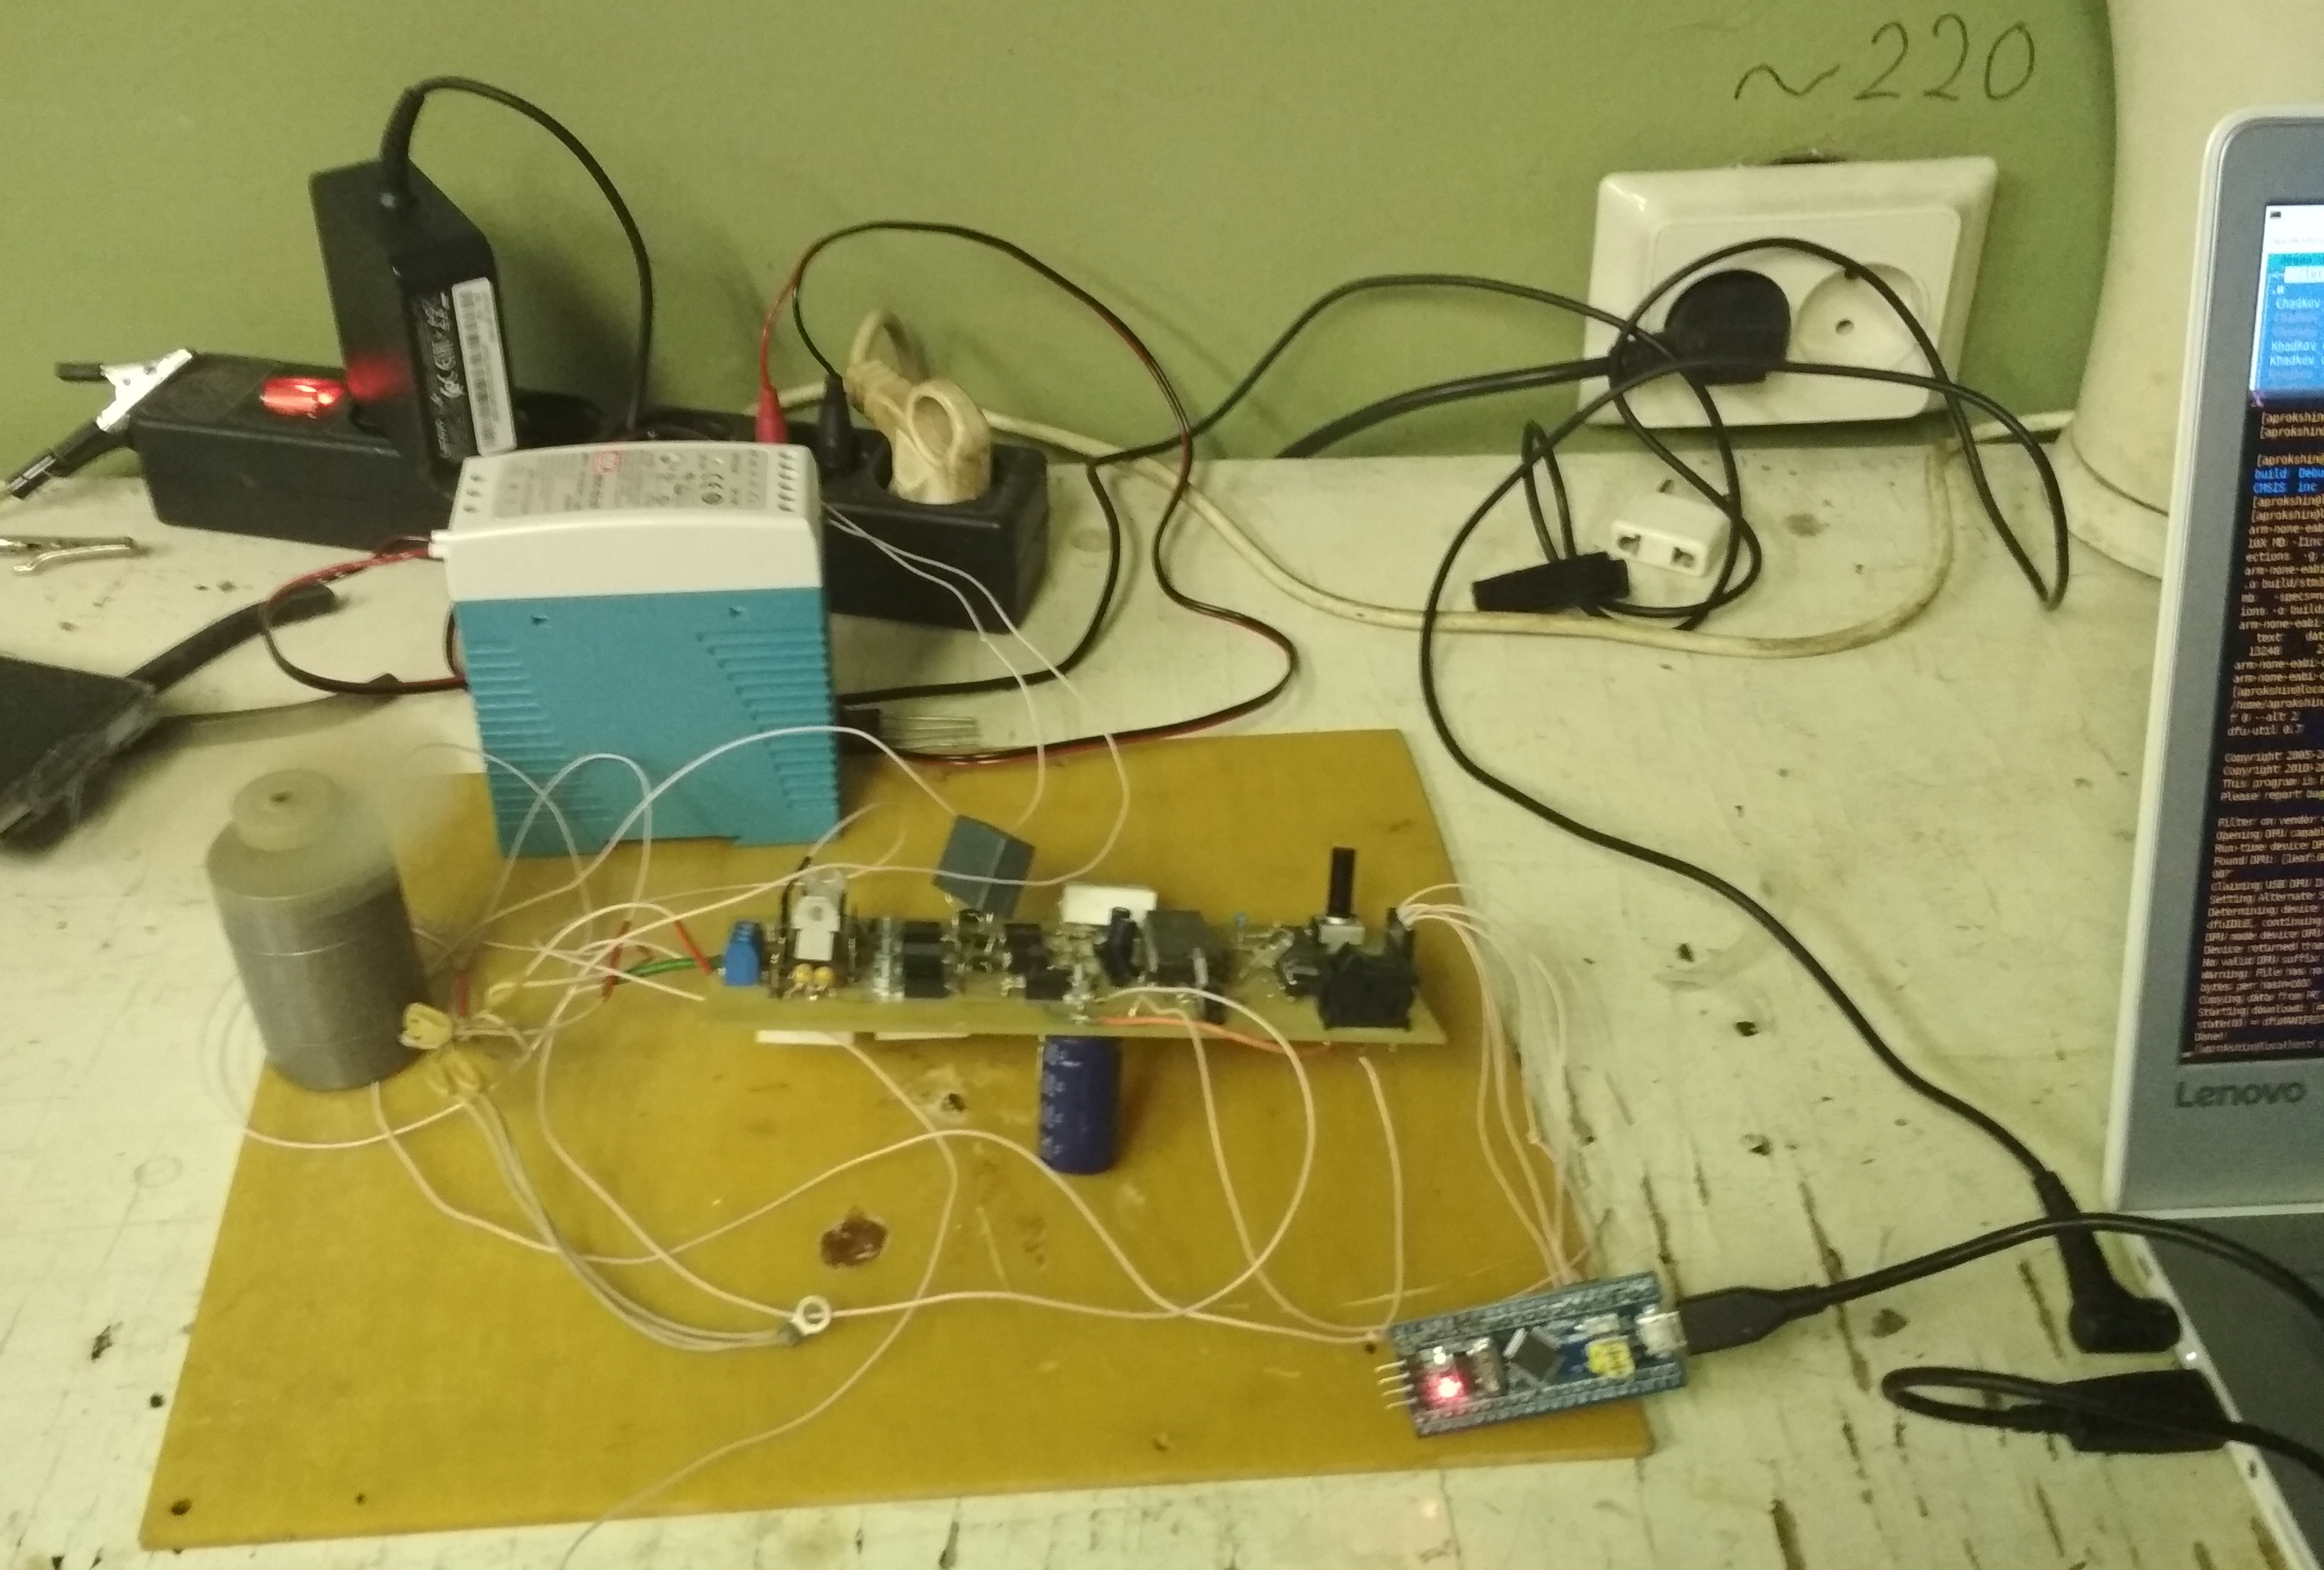
\includegraphics[width=1\linewidth]{ustanovka.jpg}}  \\
%\end{minipage}
\end{center}
\end{figure}

\end{frame}

\end{document}

